Interpreted systems are a standard semantics for describing multi-agent systems
[Fagin et al., 1995b]. They provide a natural setup to interpret specifications
in a variety of languages including temporal-epistemic logic and alternating
temporal logic [Fagin et al., 1995a; Lomuscio and Raimondi, 2006].
Parameterised interpreted systems is a parametric extension of interpreted
systems put forward to reason about unbounded multi-agent
systems~\cite{KouvarosLomuscio15b}. The parameter in a system of this kind
denotes the number of agents composing the system, each homogeneously
constructed from an agent template. We here extend parameterised interpreted
systems to Parameterised Neural-symbolic Interpreted Systems (PNIS), where the
template for the agents is not purely symbolic but it comprises a perception
mechanism that is implemented via neural networks and which is coupled with a
symbolic action mechanism. This neural-symbolic treatment of the agents follows
the Neural Interpreted Systems (NIS) model from~\cite{Akintunde+20b}.
Differently from NPIS however, NIS are limited to standard non-parametric
systems with a pre-defined number of agents.

A PNIS consists of the descriptions of an agent template, from which an
unbounded number of concrete agents may be constructed, and an environment in
which the agents operate. The agent template is defined by the following. 

\begin{definition}[Agent template.]
An {\em agent template} is a tuple $\ag t = \tuple{\lstates t, \init t, \obs t,
\acts t, \prot t, \tr t }$, where:
\begin{itemize}
  \item $\lstates t = \prvs t \times \pers t$ is a nonempty (possibly infinite)
  set of local states.  Each local state  is a pair $\tuple{\prv t, \per t}$ of
  a private state $\prv t \in \prvs t \subseteq \mathbb R^{m_{prv}}$ and a
  percept $\per t \in \pers t \subseteq \mathbb R^{m_{per}}$ that encodes the
  perception a agent has about the environment.  

  \item $\init t \in \lstates t$ is the unique initial template state.
  
  \item $\obs t : \lstates t \times \lstates e \rightarrow \pers t$ is an
  observation function that maps pairs of template local states $\lstates t
  \subseteq \mathbb{R}^{m_{prv} + m_{per}}$ and environment states $\lstates e
  \subseteq \mathbb{R}^{m_e}$ (defined below) to percepts $\pers t \subseteq
  \mathbb{R}^{m_{per}}$. The observation function is implemented via a PWL FFNN $f :
  \mathbb{R}^{m_{prv} + m_{per} + m_e} \rightarrow \mathbb{R}^{m_{per}}$.

  \item $\acts t$ is a nonempty and finite set of actions.
  
  \item $\prot t : \lstates t \rightarrow 2^{\acts t} \setminus \set{\emptyset}$
  is a local protocol function that selects which actions may be performed at a
  given local state.%%\nb{E: shouldn't the protocol take as input $\pers{t}$?}

  \item $\tr t: \lstates t \times \acts t \times 2^{\acts t} \times \acts e 
  \rightarrow \prvs t$ is a local transition function  that determines the next
  private state for a concrete agent given its current local state, its action, 
  the set of actions performed by all the agents  and the action of the
  environment.
  
\end{itemize}  
\end{definition}

% \begin{example}
%   \label{ex:agent-template}
%   We consider the example of a guarding game, an instance of sequential social
%   dilemma games \cite{LeiboZLMG17}.\nb{E: check if this is really an SSD} In this game there is a colony of
%   agents. The colony needs to be guarded by exactly one guard. Guarding duty
%   costs the guard some health, $G_p$, while those who are resting improve their
%   health by $R_r$, where the health is limited by a maximum value $M_h$. If no
%   one is guarding the colony, then all the agents in the colony lose some
%   health, $U_p$. When an agent does not have any health left, it
%   \emph{expires}.

%   We formalise the agent template
%   $\ag t = \tuple{\lstates{t}, \init{t}, \obs{t}, \acts{t}, \prot{t}, \tr{t} }$
%   in this game as follows.

 
%   \begin{itemize}[$\bullet$]
%   \item
%     $\lstates{t} = \{(h,\per{}) \mid h \in \{0,\dots,M_h\}, \ \per{} \in \{G_s,
%     R_s, E_s\}$, where $h$ is an integer between 0 and $M_h$, denoting the
%     health of the agent, while percepts $G_s$, $R_s$ and $E_s$ indicate what
%     actions are available to the agent depending on its health.
%     % stand for \emph{G}uarding, \emph{R}esting and \emph{E}xpired
%     % \emph{s}tates, respectively.

%   \item $\init{t} = (G_p + 1, G_s)$, i.e., at the start each agent has enough
%     of health to be able to guard at least once without expiring.
    
%   \item $\acts{t} = \{G_a, R_a, E_a\}$, where $G_a$, $R_a$ and $E_a$ stand for
%     \emph{G}uarding, \emph{R}esting and \emph{E}xpired \emph{a}ctions,
%     respectively.
  

%   \item Normally, we assume that the observation function is given as a
%     FFNN. But for the sake of illustration, we define here the observation
%     function of a perfectly altruistic agent:

%     $\obs{t}((h,\per{}), \ \lstate{e}) = \left\{
%       \begin{array}{rl}
%         G_s, & \text{ if } h > G_p\\ 
%         R_s, & \text{ if } 0 < h \leq G_p\\ 
%         E_s, & \text{ if } h \leq 0\\
%       \end{array} \right.$
    
%     Intuitively, if health is good enough, then the agent is in a position to
%     guard, if health is still positive, the agent can only rest, otherwise the
%     agent is ``expired''. In this example, the environment state is ignored by
%     the observation function.
    
%   \item $\prot{t}(h,\per{}) = \left\{
%       \begin{array}{rl}
%         \{G_a, R_a\}, & \text{ if } \per{} = G_s\\ 
%         \{R_a\}, & \text{ if } \per{} = R_s\\ 
%         \{E_a\}, & \text{ if } \per{} = E_s\\
%       \end{array} \right.$

%     If the percept is $G_s$, then the agent can both guard and rest. If the
%     percept is $R_s$ or $E_s$, the only available actions are resting and the
%     dummy action $E_a$, respectively.
    
%   \item The local transition function ensures that at most one agent guards at
%     any moment. Formally, for $S \in \{G_s,R_s\}$:

%     %% no restriction on everybody guarding
%     %% suitable for existential properties only
%     $\begin{array}{@{}l@{\quad}l}\small
%        \tr{t}((h,S), G_a, A) = \max(h - G_p,0) &\\% \text{ and } h > G_p\\
%        % \tr{t}((h,S), G_a, A) = 0     &\text{ if }G_a\notin A \text{ and } h \leq G_p\\[2mm]
%        \tr{t}((h,S), R_a, A) = \min(h + R_r, M_h) &\text{ if }G_a\in A\\
%        \tr{t}((h,S), R_a, A) = \max(h - U_p,0) &\text{ if }G_a\notin A\\% \text{ and } h > U_p\\
%        % \tr{t}((h,S), R_a, A) = 0     &\text{ if }G_a\notin A \text{ and } h \leq U_p\\[2mm]
       
%        \tr{t}((h,E_s), E_a, A) = h\\
%      \end{array}$

%      %% restrictions on everybody guarding or resting.
%      %% suitable for universal properties as well
%      $\begin{array}{@{}l@{\quad}l}\small
%         \tr{t}((h,S), G_a, A) = \max(h - G_p,0) &\text{ if }R_a \text{ or }S_a\text{ in } A\\% \text{ and } h > G_p\\
%         \tr{t}((h,S), G_a, A) = -1 &\text{ if }\{G_a\} = A\\% \text{ and } h > G_p\\
%         % \tr{t}((h,S), G_a, A) = 0     &\text{ if }G_a\notin A \text{ and } h \leq G_p\\[2mm]
%        \tr{t}((h,S), R_a, A) = \min(h + R_r, M_h) &\text{ if }G_a\in A\\
%        \tr{t}((h,S), R_a, A) = \max(h - U_p,0) &\text{ if }G_a\notin A\\% \text{ and } h > U_p\\
%        % \tr{t}((h,S), R_a, A) = 0     &\text{ if }G_a\notin A \text{ and } h \leq U_p\\[2mm]
       
%        \tr{t}((h,E_s), E_a, A) = h\\
%      \end{array}$
% \end{itemize}

% \end{example}

\begin{example}
      %% no restriction on everybody guarding
    %% suitable for existential properties only

  \label{ex:agent-template}

  Version 1, Everybody can guard and rest
  
  We consider the example of a guarding game, an instance of sequential social
  dilemma games \cite{LeiboZLMG17}.\nb{E: check if this is really an SSD} In
  this game there is a colony of agents. The colony needs to be
  guarded. Guarding duty costs the guard some health~$G_p$, while those who
  are resting improve their health by $R_r$, where the health is limited by a
  maximum value $M_h$. If no one is guarding the colony, then all the agents in
  the colony lose some health, $U_p$. When an agent does not have any health
  left, it \emph{expires}.

  We formalise the agent template
  $\ag t = \tuple{\lstates{t}, \init{t}, \obs{t}, \acts{t}, \prot{t}, \tr{t} }$
  in this game as follows.

 
  \begin{itemize}[$\bullet$]
  \item
    $\lstates{t} = \{(h,\per{}) \mid h \in \{0,\dots,M_h\}, \ \per{} \in \{G_s,
    R_s, E_s\}$, where $h$ is an integer between 0 and $M_h$, denoting the
    health of the agent, while percepts $G_s$, $R_s$ and $E_s$ indicate what
    actions are available to the agent depending on its health.
    % stand for \emph{G}uarding, \emph{R}esting and \emph{E}xpired
    % \emph{s}tates, respectively.

  \item $\init{t} = (G_p + 1, G_s)$, i.e., at the start each agent has enough
    of health to be able to guard at least once without expiring.
    
  \item $\acts{t} = \{G_a, R_a, E_a\}$, where $G_a$, $R_a$ and $E_a$ stand for
    \emph{G}uarding, \emph{R}esting and \emph{E}xpired \emph{a}ctions,
    respectively.
  

  \item Normally, we assume that the observation function is given as a
    FFNN. But for the sake of illustration, we define here the observation
    function of a perfectly altruistic agent:

    $\obs{t}((h,\per{}), \ \lstate{e}) = \left\{
      \begin{array}{rl}
        G_s, & \text{ if } h > G_p\\ 
        R_s, & \text{ if } 0 < h \leq G_p\\ 
        E_s, & \text{ if } h \leq 0\\
      \end{array} \right.$
    
    Intuitively, if health is good enough, then the agent is in a position to
    guard, if health is still positive, the agent can only rest, otherwise the
    agent is ``expired''. In this example, the environment state is ignored by
    the observation function.
    
  \item $\prot{t}(h,\per{}) = \left\{
      \begin{array}{rl}
        \{G_a, R_a\}, & \text{ if } \per{} = G_s\\ 
        \{R_a\}, & \text{ if } \per{} = R_s\\ 
        \{E_a\}, & \text{ if } \per{} = E_s\\
      \end{array} \right.$

    If the percept is $G_s$, then the agent can both guard and rest. If the
    percept is $R_s$ or $E_s$, the only available actions are resting and the
    dummy action $E_a$, respectively.
    
  \item The local transition function ensures that at most one agent guards at
    any moment. Formally, for $S \in \{G_s,R_s\}$:

    $\begin{array}{@{}l@{\quad}l}\small
       \tr{t}((h,S), G_a, A) = \max(h - G_p,0) &\\% \text{ and } h > G_p\\
       % \tr{t}((h,S), G_a, A) = 0     &\text{ if }G_a\notin A \text{ and } h \leq G_p\\[2mm]
       \tr{t}((h,S), R_a, A) = \min(h + R_r, M_h) &\text{ if }G_a\in A\\
       \tr{t}((h,S), R_a, A) = \max(h - U_p,0) &\text{ if }G_a\notin A\\% \text{ and } h > U_p\\
       % \tr{t}((h,S), R_a, A) = 0     &\text{ if }G_a\notin A \text{ and } h \leq U_p\\[2mm]
       
       \tr{t}((h,E_s), E_a, A) = h\\
     \end{array}$

\end{itemize}

\end{example}

% \begin{example}
%      %% restrictions on everybody guarding or resting.
%      %% suitable for universal properties as well
%   \label{ex:agent-template2}
%   Version 2
  
%   We consider the example of a guarding game, an instance of sequential social
%   dilemma games \cite{LeiboZLMG17}.\nb{E: check if this is really an SSD} In this game there is a colony of
%   agents. The colony needs to be guarded by exactly one guard. Guarding duty
%   costs the guard some health, $G_p$, while those who are resting improve their
%   health by $R_r$, where the health is limited by a maximum value $M_h$. If no
%   one is guarding the colony, then all the agents in the colony lose some
%   health, $U_p$. When an agent does not have any health left, it
%   \emph{expires}.

%   We formalise the agent template
%   $\ag t = \tuple{\lstates{t}, \init{t}, \obs{t}, \acts{t}, \prot{t}, \tr{t} }$
%   in this game as follows.

 
%   \begin{itemize}[$\bullet$]
%   \item
%     $\lstates{t} = \{(h,\per{}) \mid h \in \{0,\dots,M_h\}, \ \per{} \in \{G_s,
%     R_s, E_s\}$, where $h$ is an integer between 0 and $M_h$, denoting the
%     health of the agent, while percepts $G_s$, $R_s$ and $E_s$ indicate what
%     actions are available to the agent depending on its health.
%     % stand for \emph{G}uarding, \emph{R}esting and \emph{E}xpired
%     % \emph{s}tates, respectively.

%   \item $\init{t} = (G_p + 1, G_s)$, i.e., at the start each agent has enough
%     of health to be able to guard at least once without expiring.
    
%   \item $\acts{t} = \{G_a, R_a, E_a\}$, where $G_a$, $R_a$ and $E_a$ stand for
%     \emph{G}uarding, \emph{R}esting and \emph{E}xpired \emph{a}ctions,
%     respectively.
  

%   \item Normally, we assume that the observation function is given as a
%     FFNN. But for the sake of illustration, we define here the observation
%     function of a perfectly altruistic agent:

%     $\obs{t}((h,\per{}), \ \lstate{e}) = \left\{
%       \begin{array}{rl}
%         G_s, & \text{ if } h > G_p\\ 
%         R_s, & \text{ if } 0 < h \leq G_p\\ 
%         E_s, & \text{ if } h \leq 0\\
%       \end{array} \right.$
    
%     Intuitively, if health is good enough, then the agent is in a position to
%     guard, if health is still positive, the agent can only rest, otherwise the
%     agent is ``expired''. In this example, the environment state is ignored by
%     the observation function.
    
%   \item $\prot{t}(h,\per{}) = \left\{
%       \begin{array}{rl}
%         \{G_a, R_a\}, & \text{ if } \per{} = G_s\\ 
%         \{R_a\}, & \text{ if } \per{} = R_s\\ 
%         \{E_a\}, & \text{ if } \per{} = E_s\\
%       \end{array} \right.$

%     If the percept is $G_s$, then the agent can both guard and rest. If the
%     percept is $R_s$ or $E_s$, the only available actions are resting and the
%     dummy action $E_a$, respectively.
    
%   \item The local transition function ensures that at most one agent guards at
%     any moment. Formally, for $S \in \{G_s,R_s\}$:


%      $\begin{array}{@{}l@{\quad}l}\small
%         \tr{t}((h,S), G_a, A) = \max(h - G_p,0) &\text{ if }R_a \text{ or }S_a\text{ in } A\\% \text{ and } h > G_p\\
%         \tr{t}((h,S), G_a, A) = -1 &\text{ if }\{G_a\} = A\\% \text{ and } h > G_p\\
%         % \tr{t}((h,S), G_a, A) = 0     &\text{ if }G_a\notin A \text{ and } h \leq G_p\\[2mm]
%        \tr{t}((h,S), R_a, A) = \min(h + R_r, M_h) &\text{ if }G_a\in A\\
%        \tr{t}((h,S), R_a, A) = \max(h - U_p,0) &\text{ if }G_a\notin A\\% \text{ and } h > U_p\\
%        % \tr{t}((h,S), R_a, A) = 0     &\text{ if }G_a\notin A \text{ and } h \leq U_p\\[2mm]
       
%        \tr{t}((h,E_s), E_a, A) = h\\
%      \end{array}$
% \end{itemize}

% \end{example}

% \begin{example}\em
%   \label{ex:penguin-agent-template}
%   We consider the example of a penguin colony, an instance of sequential social
%   dilemma games \cite{LeiboZLMG17}.\nb{E: check if this is really an SSD} In
%   this scenario, there is a colony of penguins living in a very cold
%   environment. For a penguin to survive, it needs to maintain its body
%   temperature within a certain interval: if the body temperature drops too low
%   and raises too high, the penguin dies (here we assume a simplification of the
%   real-life dynamics).

%   We assume that penguins live on a
%   hexagonal grid. Given the cell where a penguin is located, there are 6
%   neighbouring cells (thus, there can be at most 6 neighbours). 

%   \def\r{3}%4}
%   \def\d{6}%8}
%   \def\w{5.2}%6.93} % r * sqrt(3)
%   \newcommand{\coord}[3]{\textcolor{purple}{#1},\! \textcolor{teal}{#2},\! \textcolor{violet}{#3}}
%   \begin{center}
%     \begin{tikzpicture}[%
%       hexagon/.style={draw=gray,  regular polygon, regular polygon
%         sides=6, minimum height=#1, rotate=30},
%       hexagon/.default={6mm}]     
%       \foreach \x in {1,2,...,4} { %
%         \foreach \y in {1,2} { %
%           \node[hexagon] at (\x*\w mm,\y*3*\r mm) {};
          
%           \node[hexagon] at (0.5*\w mm + \x*\w mm,1.5*\r mm+\y*3*\r mm) {};
%           % 
%         }}

%       \begin{scope}[xshift=5cm, yshift=1.5cm]
%         \node[hexagon=8mm] {};

%         % \node[scale=0.5] {\coord{0}{0}{0}};

%         \foreach \a/\n/\q/\r/\s in {%
%           60 /1/ 1/-1/ 0,%
%           0  /2/ 1/ 0/-1,%
%           300/3/ 0/ 1/-1,%
%           240/4/-1/ 1/ 0, %
%           180/5/-1/ 0/ 1, %
%           120/6/ 0/-1/ 1%
%         } {%
%           \node[hexagon=8mm] at (\a:6.93 mm) {};
          
%           \node[scale=0.5] at (\a:7.7 mm) {\n};%\coord{\q}{\r}{\s}};
          
%           \draw[-latex] (\a:0.25cm) -- (\a:0.55cm);%
%         }
%       \end{scope}
%     \end{tikzpicture}
%   \end{center}

%   We assume cube coordinates \cite{Patel21} for encoding the locations on the
%   hexagonal grid. Such coordinate system allows for standard vector operations,
%   for instance, given a current location $c$ and a vector of movement $a$, we
%   can compute the resulting location as $c+a$ (although in the example we
%   abstract away the exact coordinates). Assume that
%   $\mathit{Loc} \subseteq \mathbb{Z}^3$ is the arena, a set of connected
%   locations each identified by a 3d coordinate.

%   Penguins radiate heat in each of the 6 directions where there are no
%   neighbours, while for each direction where there is a neighbour the penguin
%   gains/preserves some heat. Let $r$ be the amount of heat radiated in one
%   direction. We assume the following update function for the temperature of a
%   penguin with $n$ neighbours:
%   $\mathit{upd}(t,n) = t - (6-n)\cdot r + n\cdot\frac{r}{2}$.
%   %
%   We number the directions 1 to 6 as in the figure
%   above, and denote the corresponding vectors as $v_1,\dots,v_6$. Let
%   $D = \{1,\dots,6\}$ be the set of all 6 directions.


%   We formalise the agent template
%   $\ag t = \tuple{\lstates{t}, \init{t}, \obs{t}, \acts{t}, \prot{t}, \tr{t} }$
%   in this scenario as follows.

 
%   \begin{itemize}[$\bullet$]
%   \item
%     $\lstates{t} = \{(c,t,f) \mid c \in \mathit{Loc}, \ t \in \mathbb{Z}, \ f
%     \in 2^D$, where $c$ is a 3d coordinate, $t$ an integer between 0 and $M_t$,
%     denoting the temperature of the penguin, while $f$ is a percept that is a
%     set of \emph{free} directions, indicating what neighbouring cells are
%     empty.

%   \item $\init{t} = ((0,0,0),t_0, D)$, the penguin has no neighbours.
    
%   \item $\acts{t} = \mathit{Loc}$, the actions encode the new location of a
%     penguin. % $\cup \{s\}$, where $m_l$
%     % is the action for moving to the location $l$ and $s$ for not moving.

%   \item $\obs{t}((c,t,f), \ \lstate{e}) = freedir(c,\lstate{e})$ (we will
%     define the environment state the function below)..
    
    
%   \item $\prot{t}(c,t,f) = \left\{
%       \begin{array}{rl}
%         \{c + v_i \mid i \in f\}, & \text{ if } f \neq \emptyset\\ 
%         \{c\}, & \text{ if } f = \emptyset\\ 
%       \end{array} \right.$

    
%   \item $\tr{t}((c,t, f), a, A, \act{e}) = (a, \mathit{upd}(t,n))$, where
%     $n = 6 - |f|$, i.e., the transition function updates the location and the
%     temperature of the penguin.
%   \end{itemize}

% \end{example}



An environment template has a similar description to an agent template but does
not include a perception mechanism.

\begin{definition}[Agent environment.]
An {\em agent environment} is a tuple $\ag e = \tuple{\lstates e, \acts e, \prot
e, \tr e }$, where $\lstates e  \subseteq \mathbb R^{m_e}$ is a nonempty
(possibly) infinite set of local states, $\acts e$ is a nonempty and finite set
of actions,  $\prot e : 2^{\acts e} \setminus \set{\emptyset}$ is a local
protocol function, and $\tr e : \lstates e \times \acts e \times 2^{\acts t} 
\rightarrow \lstates e$ is a local transition function.
\end{definition}

\begin{example}
  For the penguin scenario, the environment $e$ is defined as
  $\tuple{\lstates{e}, \acts{e}, \prot{e}, \tr{e}}$, where
  \begin{itemize}[$\bullet$]
  \item $\lstates{e} = \{(c,b) \mid c \in \mathit{Loc}, b\in\{0,1\}\}$. Thus
    every state is a map indicating whether there is at least one or no
    penguins at a location.
  \item $\acts{e} = \{0\}$
  \item $\prot{e} = ..$
  \item
    $\tr{e}(\mathit{map}, \act{e}, A) = A \times \{1\} \ \cup \
    (\mathit{Loc}\setminus A) \times \{0\}$ the transition function computes
    the new map, given the set of penguin actions.
  \end{itemize}
\end{example}

Agent and environment templates define the main formal structure we will be
using in this paper.

\begin{definition}[Parameterised Neural Interpreted System]
  A {\em Parameterised Neural Interpreted System} (PNIS) is a tuple $\mathcal S
  = \tuple{\ag t, \ag e, \ell}$, where $\tlabel{} : \atprop \rightarrow
  2^{\lstates t}$ is a labelling function on the agent  template states for a set
  $\atprop$ of atomic propositions.
\end{definition}

\begin{example}
  \label{ex:pnis}
  Consider the agent template in Example~\ref{ex:agent-template}.

  Assume that $e$ is.. %any environment (it is irrelevant for this example).
  
  Suppose $\atprop = \{\mathsf{a}, \mathsf{d}\}$, where $\mathsf{a}$ stands for
  alive and $\mathsf{d}$ for dead. Then we can define the labelling function
  $\ell$ as $\ell(\mathsf{a}) = \{(h,S) \mid h > 0 \text{ and }S \neq E_s\}$
  and $\ell(\mathsf{d}) = \lstates{t} \setminus \ell(\mathsf{a})$.
\end{example}

A PNIS $\mathcal S$ gives a parametric description of an unbounded collection
of {\em concrete} NIS. In particular, for any value $n \geq 1$ of the parameter
the concrete system $\sys n$ composes~$n$ copies $\ag 1, \ldots, \ag n$ of the
agent template with the environment $\ag e$. We write $\agents n$ for the set
$\agents n = \set{\ag 1, \ldots, \ag n}$ of concrete agents instantiated from
$\ag t$.
%
A \emph{global state} $q = \tuple{\lstate 1, \ldots, \lstate n, \lstate e}$ in
$\sys n$ is a tuple of local states for all the agents and the environment in
$\sys n$; it describes the system at a particular instant of time.  For a
global state $g$, we write $\lprv{a}{q}$, $\lper{a}{q}$ and $\ls{a}{q}$ to
denote the \emph{private part} $\prv a$ and the \emph{perception part} $\per a$
of the local state $\ls{a}{g} = \tuple{\prv a, \per a}$ of agent $\ag a$ in
$g$.  The set $\globalstates{n}=\lstates{1}\times\dots\times\lstates{n}\times L_e$
of all possible global states is the Cartesian product of the agents' sets of
local states.
% 
A \emph{joint action} $\alpha = \tuple{\alpha_1, \ldots, \alpha_n, \alpha_e}$
in $\sys n$ is a tuple of local actions for all the agents and the environment.
For a joint action $\alpha$, we write $\la{a}{\alpha}$ to denote the
\emph{local action} of agent $\ag a$ in~$\alpha$.  The set
$\globalacts{n} = \acts{1}\times\dots\times\acts{n}\times\acts{e}$ of all
possible joint actions is the Cartesian product of the agents' sets of local
actions.  A concrete system's global states evolve over time in compliance with
the following global transition relation.

% , i.e., for each agent $a \in \set{1,\ldots,n}$ we have that $a =
% \tuple{\lstates a, \init a, \obs a, \acts a, \prot a, \tr a} = \ag t$, 

\begin{definition}[Concrete Neural Interpreted System]
  \label{def:concreteystem}
Given an NPIS $\mathcal S = \tuple{\ag t, \ag e, \ell_t}$ and $n \geq 1$, a
\emph{concrete neural interpreted system} is a tuple $\sys n = \tuple{ \set{\ag 1,
\ldots, \ag n, \ag e}, \globalinit n, \valuation n}$, where $\globalinit n =
\tuple{\init 1, \ldots, \init n, \init e}$ is the initial global state and
$\valuation n :  \atprop \times \set{1, \ldots, n } \rightarrow 2^{\globalstates
n}$ is the concrete labelling function satisfying $q \in \valuation n(p,a)$ iff
$\ls{a}{q} \in \tlabel a(p)$.
\end{definition}

So the atomic propositions in a concrete system are indexed by each of the
concrete agents: $(p, a)$ holds in a global state if the agent $a$ is at a local
state labelled with $p$ by the template labelling function. This will enable us
to construct specifications independently of the size of the concrete system on
which they are evaluated.

Given the current global state $\tuple{\lstate 1, \ldots, \lstate n, \lstate
e}$, where $\lstate a = \tuple{\prv a, \per a}$ for $a \in \agents n$, of the
agents and the environment, the operational cycle of the agents is described as
follows. First, every agent $\ag a \in \agents n \cup \set{\ag e}$ selects an
action~$\act{a}$ that is permitted by its protocol, i.e., $\act{a} \in \prot{a}
(\lstate a)$. Then, the agents synchronously perform the selected actions.
Following  the execution of the actions each agent $\ag a \in \agents n$ updates
the private component of its local state as per its local transition function to
$\pprv a = \tr{a}( \lstate{a}, \act{a}, A, \act{e})$, where
$A = \set{ \act b \mid b \in \set{1, \ldots, n}}$.  This
generates an intermediate local state $\plstate{a} = \tuple{\pprv a, \per a}$
for each of the agents. Similarly, the environment updates its local state to
$\plstate e$. Finally, every agent $\ag a \in \agents n$ observes the update on
its local state and the update on the local state of the environment via its
neural perception module $\obs a$, thus generating a percept
$\pper a = \obs a(\plstate a, \plstate e)$, with which it updates its
perception part thereby obtaining a new local state
$\pplstate a = \tuple{ \pprv a, \pper{a}}$.


Differently from the standard treatment of interpreted systems and NIS, the
transition function of a concrete agent in PNIS  does not depend on the joint
action performed in the system, but it depends on the local action performed by
the  agent and on the on the set of actions performed by the rest of the agents
and the environment.  Thus, the identities of the agents are abstracted away in
a joint action, thereby reflecting the unbounded nature of PNIS. In other words,
whereas  a concrete agent can observe which actions were performed in the system
at a given time,  it cannot observe which agent or how many agents performed
each action.

We now formally define the temporal evolution of a concrete system
$\sys n$.



\begin{definition}[Global transition function] 
  \label{def:globaltransition}
  The {\em global transition function} $\globaltr n : \globalstates n
  \times \globalacts n \rightarrow \globalstates n$ of a concrete system $\sys n$
  satisfies $\globaltr n(q, \alpha) = q'$ iff the following hold:
  \begin{itemize}
  \item $\la{e}{\alpha} \in \prot{e}({\ls{e}{q}})$ and
    $\tr e(\ls{e}{q}, \la{e}{q}, A) = q'$, where
    $A = \set{\la{a}{q} \mid a \in \set{1,\ldots,n}}$; i.e., the environment’s
    action is protocol compliant and its local state is updated as per its
    local transition function w.r.t.\ the set of actions that were performed in
    the round.

  \item For all $a \in \set{1,\ldots,n}$, we have that
    $\la{a}{\alpha} \in \prot{a}(\ls{a}{q})$,
    $\tr a (\ls{a}{q}, \la{i}{\alpha}, A, \la{e}{\alpha}) = \lprv{a}{q'}$,
    where $A = \set{\la{b}{q} \mid b \in \set{1,\ldots,n}}$, and
    $\obs a((\lprv{a}{q'},\lper{a}{q}),\ls{e}{q'}) = \lper{a}{q'}$; i.e., the
    agent's action is protocol compliant, the private part of its local state
    is updated as per its local transition function w.r.t to the set of actions
    performed by all the agents, and the perception part of its local state is
    updated as per its observation function.
  \end{itemize}
\end{definition}


Each concrete system is associated with a temporal model 
that we will use  to interpret our specification language.

\begin{definition}[Model]
  \label{def:model}
  Given a concrete NIS $\sys n$, the induced model of $\sys n$, or simply model,
  is a tuple $\msys  n = \tuple{\globalstates n, \globalacts n, \globalrel n,
  \valuation n}$, where $G(n)$ is the set of global states, $\globalacts n$ is the
  set of joint actions, $\globalrel n$ is the global transition relation defined
  as $(q, \alpha, q') \in \globalrel n$ iff $\globaltr n(q, \alpha) = q'$, and 
  $\valuation n$ is the labelling function as in
  Definition~\ref{def:concreteystem}.
\end{definition}

We now illustrate Definitions~\ref{def:concreteystem}-\ref{def:model} on our running
example.

\begin{example}
  Consider a concrete neural interpreted system
  $\sys{2}=\tuple{\set{1,2,e}, \globalinit{2}, \valuation{2}}$ for the agent
  template in Example~\ref{ex:agent-template} and PNIS in
  Example~\ref{ex:pnis}, where
  $\globalinit{2} = \tuple{\init{1},\init{2}, \init{e}}$ and
  $\init{i} = (G_p+1, G_s)$. Moreover, assume that $\valuation{2}$ is defined
  from $\ell$.

  Let us assume that $G_p=R_r=1$, $U_p=2$. For brevity we omit the environment
  local state $\lstate{e}$.  The model $\msys{2}$ of $\sys{2}$ can be depicted
  as follows.

  \begin{center}
    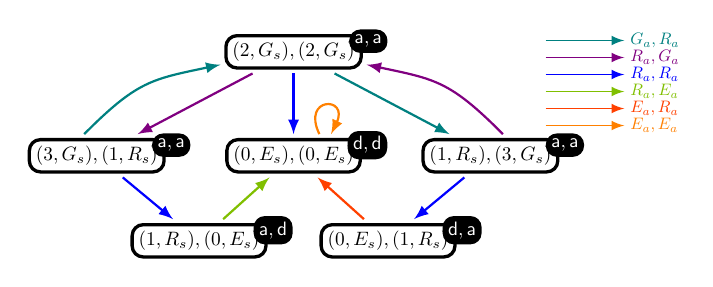
\begin{tikzpicture}[yscale=1.2, %
      gr/.style={green!50!blue}, %
      rg/.style={red!50!blue}, %
      rr/.style={blue}, %
      re/.style={green!50!orange}, %
      er/.style={red!50!orange}, %
      ee/.style={orange}, %
      ]

    \foreach \a/\hone/\perone/\htwo/\pertwo/\prop/\x/\y in { %
      s22gg/2/G_s/2/G_s/{a,a}/0/1.1,%
      s00/  0/E_s/0/E_s/{d,d}/0/0,%
      s31/  3/G_s/1/R_s/{a,a}/-2.5/0,%
      s13/  1/R_s/3/G_s/{a,a}/2.5/0,%
      s10/  1/R_s/0/E_s/{a,d}/-1.2/-0.9,%
      s01/  0/E_s/1/R_s/{d,a}/1.2/-0.9%
    }{ %
      \node[scale=0.7, outer sep=1mm,draw, very thick, rounded corners] (\a) at (\x,\y) {$(\hone,\perone), (\htwo,\pertwo)$};

      \node[fill=black, text=white, rounded corners, inner sep=1mm, scale=0.7, xshift=0.3mm, yshift=-2mm] at (\a.north east) {$\mathsf{\prop}$};
      }

      \foreach \from/\to/\lab/\wh in { %
        s22gg/s00/{rr}/left, s22gg/s31/{rg}/left, s22gg/s13/{gr}/right, %
        s31/s10/{rr}/left, %
        s13/s01/{rr}/left, %
        s10/s00/{re}/left,%
        s01/s00/{er}/right%
      }{ \draw[-latex,thick,\lab] (\from) -- (\to);
      }

      \foreach \from/\to/\out/\in/\loose/\lab/\wh in { %
        s00.40/s00.30/120/60/8/{ee}/above,%
        s31.120/s22gg.190/40/190/1.2/{gr}/right,%
        s13.60/s22gg.350/140/350/1.2/{rg}/left%
      }{%
        \draw[-latex,thick,\lab] (\from) to[out=\out,in=\in, looseness=\loose]  (\to); %
      }

      \begin{scope}[yshift=1.4cm]
      \foreach \col/\y/\lab in { %
        gr/1/{G_a,R_a}, rg/2/{R_a,G_a}, rr/3/{R_a,R_a}, %
        re/4/{R_a,E_a}, er/5/{E_a,R_a}, ee/6/{E_a,E_a}%
      }{ \draw[-latex, semithick, \col] (3.2,-0.18*\y) -- ++(1,0) node[right, scale=0.6] {$\lab$}; }
    \end{scope}
    \end{tikzpicture}
  \end{center}
 
\end{example}


A path in a model $\msys n$ is an infinite sequence of global states anc joint
actions $q^0\alpha^0q^1\alpha1\ldots$ such that $(q^i,\alpha^i,q^{i+1}) \in
\globalrel n$ for all $i \geq 0$. Given a global state $q$ in $\msys n$ we write
$\paths{q}$ for the set of all paths originating from $q$.
  
We express specifications for PNIS in an indexed and bounded variant of
Computation Tree Logic ($\ctl$), henceforth $\bictl$. The logic (i) introduces
indexed atomic propositions that are quantified over the agents of the concrete
system the formula in question is evaluated; and (ii) permits only the
construction of formulae whose evaluation can be realised on paths of bounded
lengths. The former extends $\ctl$ by allowing the formulation of properties
irrespective of the concrete system on which they are evaluated.  The latter
restrict $\ctl$ following the undecidability verification for unbounded
formulae~\cite{Akintunde+20}.

\begin{definition}
Given a  set $\atprop$ of atomic propositions and a set $\atvar$ of variables,
the $\bictl$  formulae are defined by the following BNF:
\[
  \varphi \;   ::= \; (p, v) \mid \varphi \lor \varphi \mid \varphi \land \varphi
  \mid AX^K \varphi \mid \forall v : \phi,
\]
where  $p \in \atprop$, $v \in \atvar$ and $k \geq  1$.
\end{definition}

The formula $AX^k \varphi$ is read as ``for all paths, $\varphi$ holds at the
$k$-th step''. We inductively abbreviate bounded until as
\begin{align*}
 A(\varphi U^1 \psi) &\triangleq \psi \lor (\varphi \land AX^1 \psi) \\
 A(\varphi U^k \psi) &\triangleq \psi \lor (\varphi \land AX^1 (A (\varphi U^{k-1} \psi)).
\end{align*}
with the meaning ``there is a path in which $\psi$ holds at some point in the
$k$ following steps and before then $\varphi$ is true along the path. 
% The dual
% until, prefixed by the universal operator, can be defined analogously.

A $\bictl$ formula is said to be a sentence if every variable appearing the
formula is in the scope of a universal quantifier. Hereafter we consider only
indexed $\bictl$ sentences of the form $\forall v_1 \ldots \forall v_m :
\varphi$, or, shortly, $\bictlspec$, where $v_i \in \atvar$ for $i \in
\set{1,\ldots,m}$ and $\varphi$ does not contain any universal quantifier.

We now define the satisfaction relation for $\bictl$ on the temporal models
associated with the concrete systems.

\begin{definition}[Satisfaction]
  \label{def:sat} 
  Given a model $\msys n$, a global state~$q^0$ and a $\bictl$ sentence
  $\bictlspec$ with $m \leq n$, the \emph{satisfaction} of $\varphi$ at $q$\nb{E: $q$ or $q^0$?},
  denoted $(\msys n, q) \models\varphi$, or simply $q \models \varphi$ when
  $\msys n$ is clear from the context, is defined as follows:
  \begin{description}
  \item[$q \models (p, a)$] \ iff \ $q^o \in \valuation n((p, a))$, for $p \in
  \atprop$ and $a \in \agents n$; 
  \item[$q \models \varphi \lor \psi$] \ iff \ $q \models \varphi$ or $q \models
  \psi$;
  \item[$q \models \varphi \land \psi$] \ iff \ $q \models \varphi$ and $q
  \models \psi$;
  \item[$q \models EX^k  \varphi$] \ iff  there is $\rho \in \paths{q}$ such
  that $\rho(k) \models \varphi$;
  \item[$q \models AX^k  \varphi$] \ iff for all $\rho \in \paths{q}$ we
  have that $\rho(k) \models \varphi$;
  \item[$q \models \bictlspec$] \ iff for all $h : \set{v_1, \ldots, v_m}
  \rightarrow \set{\ag 1, \ldots,\ag n}$ we have that $q \models 
  \varphi[v_1 \mapsto h(v_1), \ldots v_m \mapsto h(v_m)]$\nb{E: what is $h$? Would be good to explain it}
\end{description}
\end{definition}

A sentence $\bictlspec$ is said to be true in $\msys n$, denoted $\msys n
\models \bictlspec$ if $(\msys n, \globalinit n) \models \bictlspec$. The
sentence is said to be true in $\npis$, denoted $\npis \models \bictlspec$, if
$\bictlspec$ is true in every model induced by every concrete system
instantiated from $\npis$ with at least $m$ agents, i.e., $\forall n \geq m :
\msys n \models \bictlspec$.  The {\em parameterised verification problem} is to
check whether this holds.


\begin{definition}[Parameterised verification problem]
  Given an NPIS $\npis$ and a $\bictl$ sentence $\bictlspec$, determine whether
  $\npis \models \bictlspec$.
\end{definition}

  
  % Lomuscio, 2016b]. Given a set IND of indices, a set L AP
  % of local atomic propositions and a set G AP of global
  % atomic propositions, IACTLK\X formulae are defined by
  % the following BNF grammar:
  % φ ::= (p, v) | ¬(p, v) | q | ¬q | φ ∧ φ | φ ∨ φ | A(φU φ) |
  % A(φRφ) | Kiφ | ∀v : φ
  % where p ∈ L AP , q ∈ G AP , and v ∈ IND. The epis-
  % temic modality Kiφ is read as “agent i knows that φ”. The
  % temporal modality A(φU ψ) stands for “for all paths, at some
  % point ψ holds and before then φ is true along the path”; and
  % A(φRψ) denotes “for all paths, ψ holds along the path up to
  % and including the point when φ becomes true in the path”. An
  % IACTLK\X formula is said to be a sentence if every variable
  % appearing the formula is in the scope of a universal quantifier.
  % Hereafter we consider only indexed IACTLK\X sentences.
  % We now define the satisfaction relation.

  % We verify NIS against a bounded variant of a restricted
  % subset of ATL∗ (Alur, Henzinger, and Kupferman 2002),
  % drawing inspiration from Real Time Computation Tree
  % Logic (RTCTL) (Emerson et al. 1992). The satisfaction sta-
  % tus of the formulae expressible in our language depends only
  % on paths of a bounded length. This has been shown to be
  % practically relevant by enabling the efficient identification
  % of shallow bugs in a system’s execution (Biere et al. 2003;
  % Penczek, Wo´zna, and Zbrzezny 2002). In addition to this


  % practical consideration, our restriction to a bounded frag-
  % ment of ATL∗ follows the undecidability of the verification
  % problem for unbounded formulae (Akintunde et al. 2020a




%%% Local Variables:
%%% mode: latex
%%% fill-column: 79
%%% TeX-master: "../main"
%%% End:
